\documentclass[12pt,a4paper]{article}
\usepackage{rmpackages}																% usual packages
\usepackage{rmtemplate}																% graphic charter
\usepackage{rmexocptce}																% for DS with cptce eval

%\cfoot{} 													% if no page number is needed
%\renewcommand\arraystretch{1.5}		% stretch table line height

\begin{document}
\begin{header}
Mesurer une molécule
\end{header}

\section*{Objectif}

En vous appuyant sur l'expérience historique de Benjamin Franklin décrite ci-dessous, vous devrez répondre à la question :

\begin{objectif}
Quelle est la taille d'une molécule d'huile ?
\end{objectif}

\section*{L'expérience historique de Benjamin Franklin}

Au $\text{XVIII}^\text{ème}$ siècle, Benjamin Franklin se promène au bord de l'étang de Clapham en Angleterre, et décide de verser un peu d'huile dans l'eau. Il observe alors qu'une tache se forme à la surface et s'étend rapidement jusqu'à couvrir presque un quart de la surface du plan d'eau.

Il faudra attendre 1890 pour que Lord John Rayleigh reprenne cette expérience et en déduise la taille des molécules d'huile.

\begin{multicols}{2}
\center
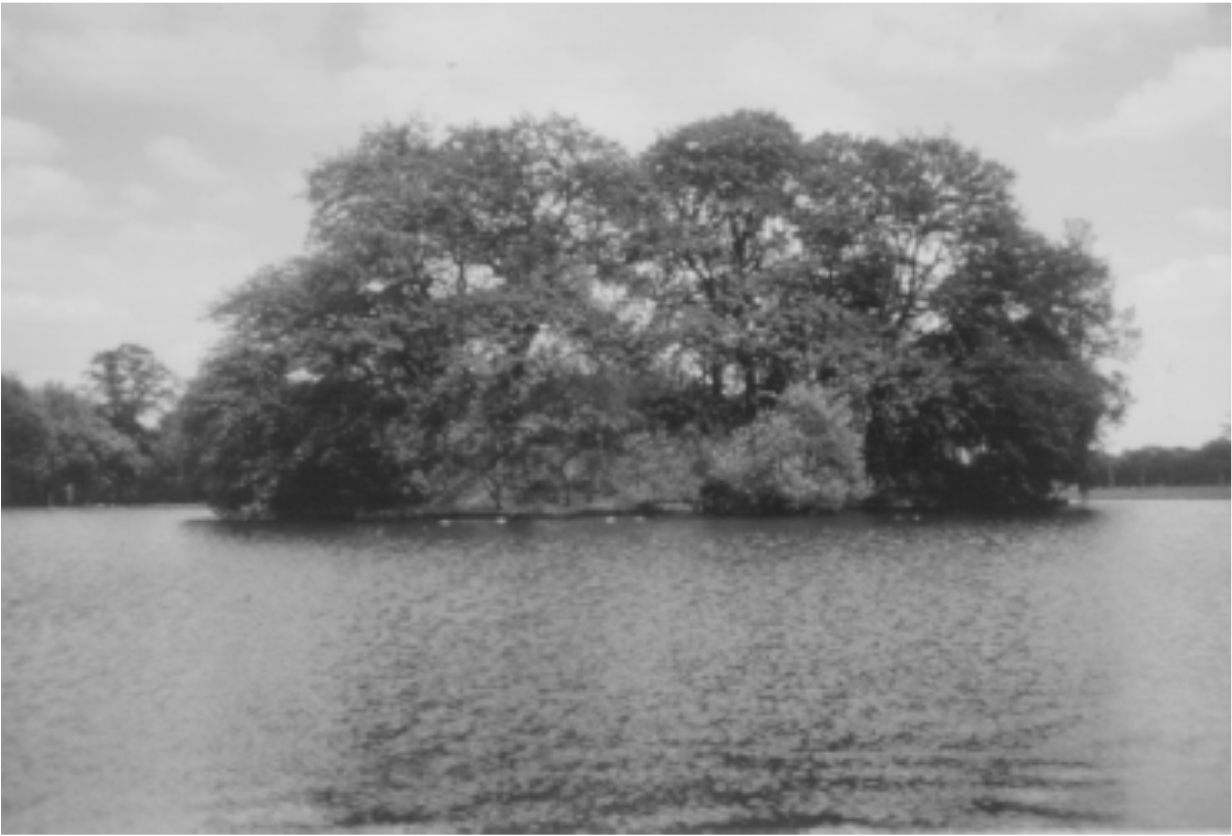
\includegraphics[height=150pt]{images/franklin_lake.png}

L'étang agité un jour venteux.

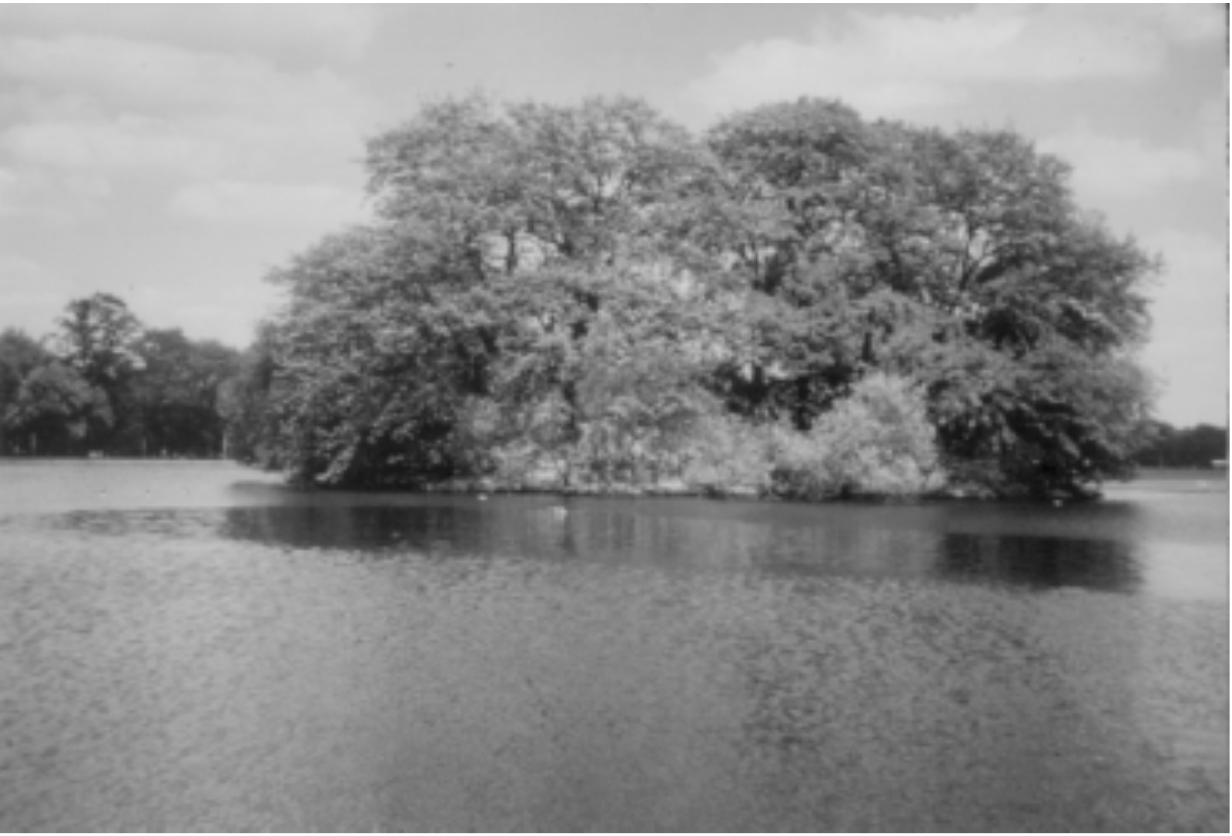
\includegraphics[height=150pt]{images/franklin_lake_oiled.png}

La tache d'huile forme une étendue lisse.
\end{multicols}

\begin{doc}
\textbf{1 : extrait d'une lettre de Benjamin Franklin à la Royal Society (1774)}
\begin{multicols}{2}
\noindent
Texte original :

\textit{ \og
At length being at Clapham where there is, on the common, a large pond, which I observed to be one day very rough with the wind, I fetched out a cruet of oil, and dropped a little of it on the water.
I saw it spread itself with surprising swiftness upon the surface ;
[...] the oil, though not more than a \textbf{tea spoonful}, produced an instant calm over a space \textbf{several yards square}, which spread amazingly and extended itself gradually till it reached the lee side, making all that quarter of the pond, perhaps half an acre, as smooth as a looking-glass.
\fg{} }

\noindent
Traduction :

Enfin à Clapham où il y a, sur la commune, un grand étang que j'observai agité un jour de grand vent, je cherchai une burette d'huile et en laissai tomber un peu sur l'eau.
Je la vis se répandre sur la surface avec une rapidité surprenante ;
[...] l'huile, bien que moins d'\textbf{une cuillère à café}, produisit un calme immédiat sur une surface de \textbf{plusieurs mètres carrés}, qui se propagea incroyablement et s'étendit progressivement jusqu'à la côte rendant ce quart de l'étang, peut-être une demie acre, aussi lisse qu'un miroir.
\end{multicols}
\end{doc}

\begin{doc}
\textbf{2 : vue aérienne de l'étang de Clapham à la fin de l'expérience de Benjamin Franklin}

\begin{center}
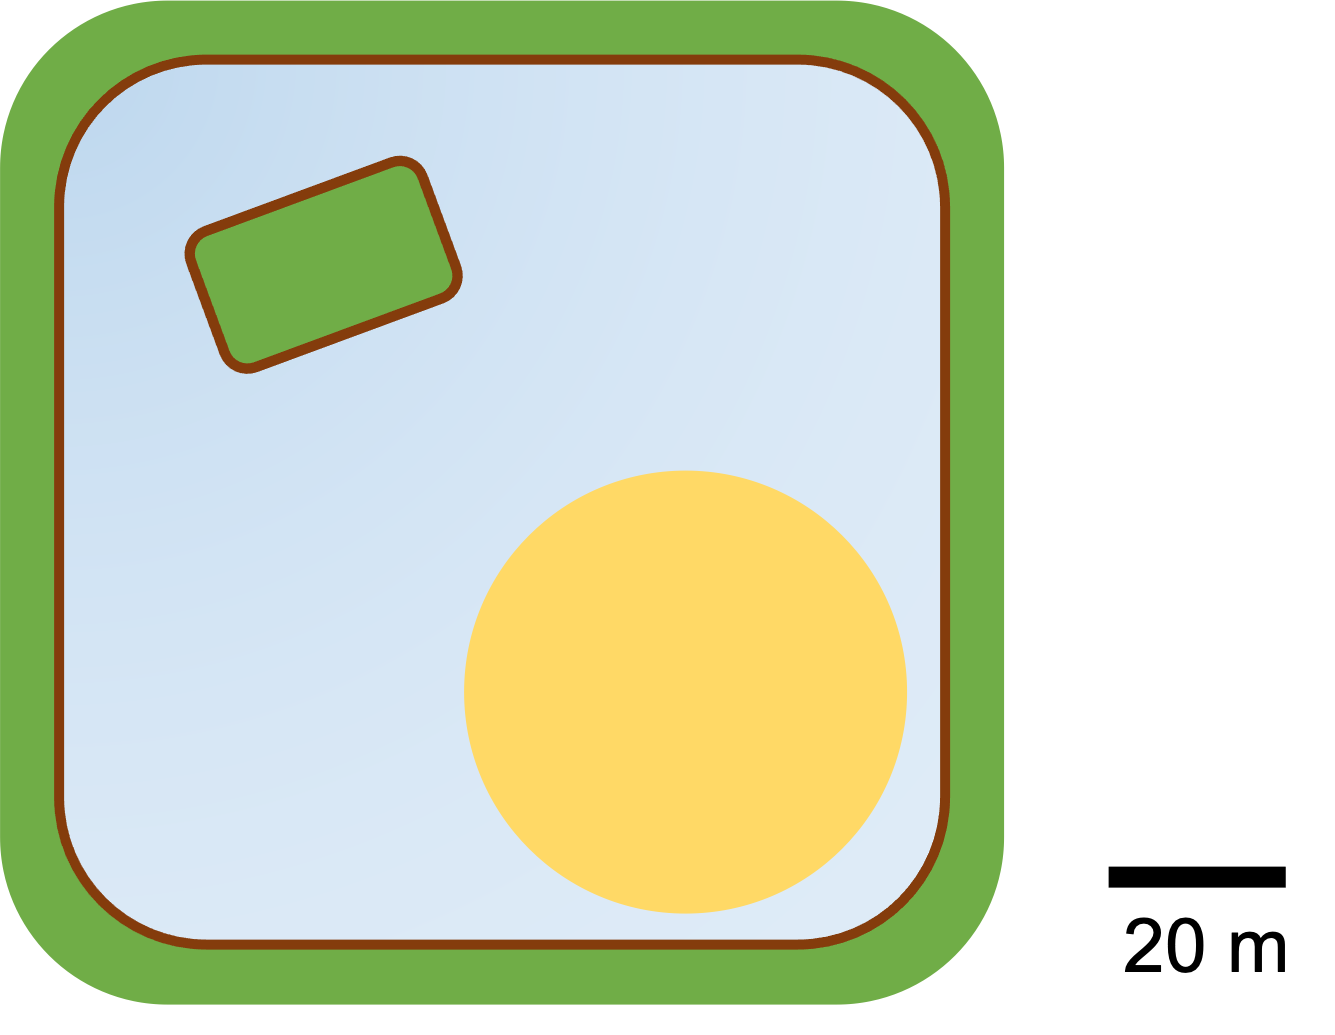
\includegraphics[scale=0.5]{images/clapham_pond.png}
\end{center}
\end{doc}

\section*{Donnée}

$ \unit{1}{mL} = \unit{1\times 10^{-6}}{m\cubed}$

\section*{Aide à la rédaction du compte-rendu}

\begin{enumerate}
\item \textbf{Hypothèse}.
Donnez votre hypothèse et justifiez-la : \og Je pense que ... car ... \fg{}.
\item \textbf{Protocole}.
Mettre en place un protocole pour vérifier votre hypothèse. Il peut contenir :
\begin{itemize}
\item[•] une expérience :
\begin{enumerate}
\item liste du matériel ;
\item schémas ;
\item observations et mesures ;
\end{enumerate}
\item[•] un calcul :
\begin{enumerate}
\item formule littérale ;
\item conversion ;
\item application numérique ;
\end{enumerate}
\item[•] un raisonnement, une étude de documents, etc.
\end{itemize}
\item \textbf{Conclusion}. Pour terminer le compte-rendu :
\begin{itemize}
\item[•] donner les conclusions en reprenant ce qui a été trouvé dans le protocole ;
\item[•] dire si les conclusions sont en accord avec votre hypothèse ;
\item[•] répondre à la question posée !
\end{itemize}
\end{enumerate}

\end{document}

\section*{Évaluation}

L'évaluation de votre travail se fera sur la base des compétences mobilisées pour répondre à la question posée.
Vous pouvez vérifiez que vous remplissez les différents critères en vous reportant à la grille ci-dessous. 

\begin{center}
\begin{tabular}{l|l}
\textbf{Compétences} & Aptitudes à vérifier \hfill \textbf{Suis-je capable de ... ?} \\
\hline
\hline
\app				 		& Me servir correctement des ressources disponibles (doc, énoncé, ...) \\
		         			& Choisir les informations qui me seront utiles \\
							& Faire un schéma de l'expérience \\
							& Évaluer quantitativement les grandeurs physiques inconnues et non précisées \\
\hline
\anarai		  		& Faire une hypothèse, la justifier \\
							& Justifier le protocole choisi \\
      						& Donner des conclusions à l'activité \\
\hline
\rea     				& Réaliser correctement les calculs analytiques et/ou numériques \\
\hline
\val		      			& Dire si mes résultats sont en accord avec ceux attendus \\
			       			& Avoir un regard critique sur mes résultats \\
\hline
\com				  	& Rendre compte de façon écrite ou orale \\
		         			& Utiliser un vocabulaire et des modes de représentation adaptés \\
\hline
\rco         			& Restituer ses connaissances \\
\end{tabular}
\end{center}